\chapter{Algorithm}
\section{Structure of a interpolation method}

In this section we will see how was implemented the interpolation method. The steps for the implementation are:

\begin{enumerate}
\item	Segmentation of metallic part on the corrupted image. 
\item	Radon transform of the corrupted image. 
\item	Identification of the inpainting domain based on the radon transform of metallic part identified 
\item	Inpainting of the domain using the interpolation technique.   \item	Filtered back projection of the inpainted sinogram 
\item	Merge of the restored image with the segmented metallic part. 
\end{enumerate}

\begin{figure}[h]
\centering
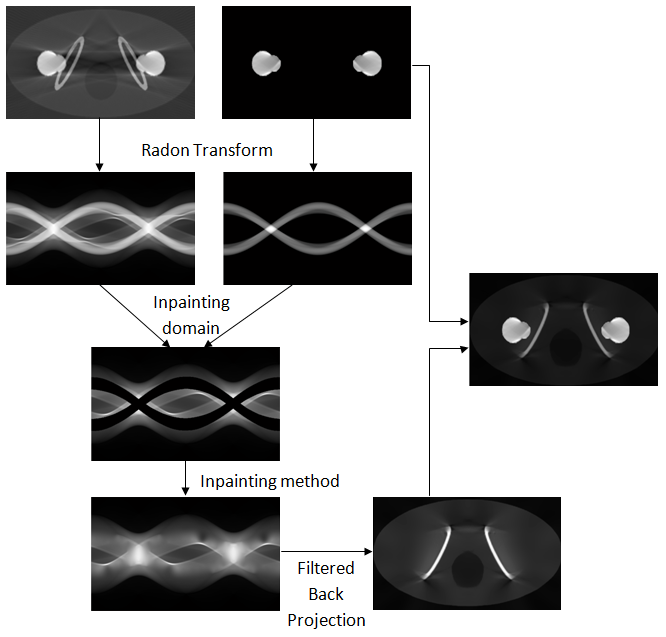
\includegraphics[scale=0.75]{img/schema}
\caption{{General Scheme}}\label{schema_fig}
\end{figure}

Except for the step 4, all of them are implemented in Matlab. The step 4 depend of the method, for the Linear interpolation we adopt only matlab, for the Interpolation of Bertalmio et al., we adopt Matlab and FreeFem++, to solve the partial differential equation.
On the next part we will explain how each step is done.

See the figure \eqref{schema_fig} for a visual model of the schema.

\section{Segmentation}

The segmentation of metallic part on the corrupted image is done using a threshold. However, this process is not enough due to some false positive, so we apply a closing morphological operator eliminating these problems. The figure \eqref{segmentation_fig} show what happen on each step.

\begin{figure}[h]
\centering
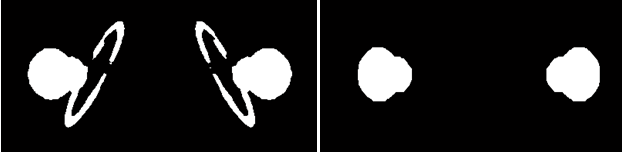
\includegraphics[scale=0.7]{img/segmentation}
\caption{{Segmentation Step. image after the threshold(left), image after closing operator(right).}}\label{segmentation_fig}
\end{figure}

\section{Radon Transform}
In Matlab there is a function that execute the Radon transform of a image. To use it we pass as parameter the image and a vector with all the angles to calculate the projections.

\section{Linear interpolating}
The linear interpolating is done taking in account the vertical extreme of the each side of domain, so a linear function is traced between them, using the function interp1 provided by Matlab. It is worth mentioning that the interpolating is done one time for each value of 'x' coordinate of the sinogram, that represent a projection angle.

\begin{figure}[h]
\centering
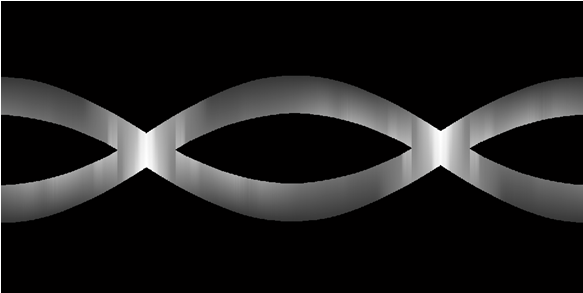
\includegraphics[scale=0.7]{img/linear_interpolation}
\caption{{A linear interpolation, we can see a discontinuity on the 'x' coordinate, because the interpolation happens only on the 'y' coordinate}}\label{linear_interpolation}
\end{figure}


\section{Bertalmio et al. interpolating}
The method of Bertalmio consist in resolve two partial differential equation. This task is divided on two great step, divided the domain in a triangular grid and solve the PDE using finite element.
To execute the triangulation we used the function DelaunayTri on Matlab, where each pixel represent a vertex of a triangle.

The function DelaunayTri request two thing: The points that will be the vertex of the triangles ( In our case all the pixel inside the inpainting domain) and the constraints, i.e, the boundary of the domain. If we don't use any constraints, the grid will be convex hull of our domain.\eqref{triangle_fig}

\begin{figure}[h]
\centering

\includegraphics[scale=1]{img/triangle}
\caption{{The triangular grid without the constraints (left) and with constraints (right)}}\label{triangle_fig}
\end{figure}

To solve the PDE which the equation is described by \eqref{NS_eq} and \eqref{vort_eq} we used the software Freefem++.

\begin{equation}\label{NS_eq}
\begin{cases}
-\nu\Delta v + v\cdot\nabla v + \nabla p = 0 & D \\
\nabla\cdot v = 0   & D \\
v(:,0) = v(:,2\pi) & D \\
v= \nabla^\bot u_{orig} & \partial D\setminus\left\lbrace(x,\theta)|\theta = 0 or \theta = 2\pi\right\rbrace \\
\nu =\frac{1}{1+\frac{\Vert\nabla^\bot u\Vert}{k}} \\
\end{cases}
\end{equation}
\begin{equation}\label{vort_eq}
\begin{cases}
\nabla^\bot u = v & D \\
u(:,0) = u(:,2\pi) & D \\
u = u_{orig} & \partial D\setminus\left\lbrace(x,\theta)|\theta = 0 or \theta = 2\pi\right\rbrace \\
\end{cases}
\end{equation}


The numerical resolution is done using the Galerkin-finity element with the fixed point approximation for the non-linearity part. The dirichlet border conditions is done with the penalty method. On the equation\eqref{vort_eq} is applied a rotational operator. The weak formulations is expressed by:

\begin{equation}\label{NS_ef}
\begin{cases}
a(v^k,w)+c(v^{k-1},v^{k},w)+b(w,p^k)=F(w) & \forall w \in V \\
b(v^k,q)=0 & \forall q \in Q \\
\end{cases}
\end{equation}
\begin{equation}\label{vort_ef}
\begin{cases}
a_2(u,\psi) = F_2(\psi) & \forall \psi \in R
\end{cases}
\end{equation}
where
\begin{align*}
V = V(D) &= \left\lbrace{w(x',\theta)|w=\Sigma_n{w_n\alpha_n(x',\theta)},w_n \in \mathbb{R},(x',\theta) \in D, w(:,0)=w(:,2\pi)} \right\rbrace \\
Q = Q(D) &= \left\lbrace{q(x',\theta)|q=\Sigma_n{q_n\beta_n(x',\theta)},q_n \in \mathbb{R},(x',\theta) \in D} \right\rbrace \\
R = R(D) &= \left\lbrace{r(x',\theta)|w=\Sigma_n{r_n\gamma_n(x',\theta)},r_n \in \mathbb{R},(x',\theta) \in D, r(:,0)=r(:,2\pi)} \right\rbrace \\
\end{align*}

\begin{align*}
a(v,w) &= \nu \int_D {\nabla v \nabla w} + \lambda  \int_{\partial D'}{vw} \\
c(u,v,w) &= \int_D  {(u\cdot\nabla)v\cdot w} \\
b(w,q) &=  -\int_D {q(\nabla\cdots w)} \\
F(w) &=  \lambda \int_{\partial D'}{v_{orig}w} \\
v_{orig} &= \nabla^\bot u_{orig} \\
a_2(u,\psi) &= \int_D {\nabla u \nabla psi} + \lambda  \int_{\partial D'}{u\psi} \\
F_2(\psi) &= -\int_D {(\nabla\times v)\psi}  + \lambda \int_{\partial D'}{u_{orig}\psi} \\
\partial D' &= \partial D\setminus\left\lbrace(x,\theta)|\theta = 0 or \theta = 2\pi\right\rbrace  \\
\end{align*}

The problems \eqref{NS_ef} and \eqref{vort_ef} are solved using finite element in P1b, for $\alpha_n (V_h)$,  P1, for $\beta_n (Q_h)$ and P2, for $\gamma_n (R_h)$.

Because of the non linearity of the problem \eqref{NS_ef},it need be solved iteratively until reach a stopping criterion. The criterion are:
\begin{itemize}
\item $  \frac{{\Vert v_k-v_{k-1}\Vert}_{H^1}}{{\Vert v_0\Vert}_{H^1}} < \varepsilon$ 
\item Maximum number of iteration
\item $  \frac{{\Vert v_k-v_{k-1}\Vert}_{H^1}}{{\Vert v_0\Vert}_{H^1}} > \beta$ (In this case the solution is diverging, so we stop the algorithm)
\end{itemize}

Each iteration use the Schur complement to create a linear system that is solved through GMRES. Additionally, a matrix need to be passed as precondition to accelerate the resolution of the linear system. We have two candidates:
\begin{itemize}
\item The matrix $Mp^{-1}$ formed by the $m(p,q)=\int_D {pq}$ where $p,q \in Q_h$
\item The diagonal matrix $M^{-1}$ formed by the diagonal elements of $Mp$
\end{itemize}

After all, the problem \eqref{vort_ef} can be solved direct.

Both problems have a Dirichlet conditions, these conditions is what associate the image inpainting with a fluid dynamics problem, thus is a high important part. The problem \eqref{vort_eq} have as 'entry' the pixel intensity of the image that is taken direct.

However, the problem \eqref{NS_eq} have as 'entry' a stream line of the pixel intensity, to calculate it we used finite different method of first order additionally a medium filter. The medium filter is necessary to reduce the noise and preventing it to alter the image inpainting.

\section{Inverting the sinogram}
To invert the sinogram we do the filtered back projection using a function called 'iradon' provided by the Matlab. Subsequently we apply a edge-preserving blur filter.

This filter is a medium filter, however instead of use all nearest pixel to calculate the mean, use only the nearest pixel with the intensity is similar, thereby, preserving the edge. Mathematically can be write like this:
\[M(i,j) = \frac{\Sigma_{p=-v}^{p=v} \Sigma_{q=-v}^{q=v} B(i+p,q+q)}{N}\]
\[B(i+p,j+q) = \begin{cases}
0 & \vert b(i+p,j+q) - b(i,j) \vert > T \\
b(i+p,j+q) & \vert b(i+p,j+q) - b(i,j) \vert < T
\end{cases} \]
where, $T$ is a threshold, $v$ a window, $b$ the pixel intensity.

Lastly we add the segmented metal part to the inverted image to obtain the restored image.


